\documentclass[aspectratio=169,11pt,xcolor=table]{beamer}

\usepackage[T1]{fontenc}
\usepackage[utf8]{inputenc}
\usepackage{helvet}
\usepackage{graphicx}
\usepackage{booktabs}
\usepackage{tabularx}
\usepackage{array}
\usepackage{ragged2e}
\usepackage{hyperref}

\renewcommand{\familydefault}{\sfdefault}
\graphicspath{{assets/}}
\urlstyle{same}

% SEGULA-inspired palette taken from the supplied official presentation.
\definecolor{Canvas}{HTML}{FFFFFF}
\definecolor{Ink}{HTML}{172033}
\definecolor{Muted}{HTML}{657286}
\definecolor{Panel}{HTML}{F1F4F6}
\definecolor{Rule}{HTML}{C7D0D8}
\definecolor{BrandBlue}{HTML}{184D6B}
\definecolor{BrandCyan}{HTML}{009BDA}
\definecolor{BrandMagenta}{HTML}{BF2F88}
\definecolor{Good}{HTML}{17865C}
\definecolor{Warn}{HTML}{E6602A}
\definecolor{Purple}{HTML}{7655C7}

\setbeamercolor{background canvas}{bg=Canvas}
\setbeamercolor{normal text}{fg=Ink,bg=Canvas}
\setbeamercolor{frametitle}{fg=BrandBlue,bg=Canvas}
\setbeamercolor{structure}{fg=BrandCyan}
\setbeamercolor{alerted text}{fg=Warn}
\setbeamercolor{footer}{fg=white,bg=BrandBlue}
\setbeamercolor{title panel}{fg=white,bg=BrandBlue}

\setbeamerfont{normal text}{size=\fontsize{11.2}{13.4}\selectfont}
\setbeamerfont{frametitle}{size=\fontsize{18.5}{21}\selectfont,series=\bfseries}
\setbeamerfont{title}{size=\fontsize{27}{30}\selectfont,series=\bfseries}
\setbeamerfont{subtitle}{size=\fontsize{12.5}{15}\selectfont}

\setbeamersize{text margin left=0.78cm,text margin right=0.78cm}
\setbeamertemplate{navigation symbols}{}
\setbeamertemplate{itemize item}{\color{BrandCyan}\raise0.18ex\hbox{\rule{0.55ex}{0.55ex}}}
\setbeamertemplate{itemize subitem}{\color{BrandCyan}\raise0.18ex\hbox{\rule{0.42ex}{0.42ex}}}
\setlength{\leftmargini}{1.25em}

\setbeamertemplate{frametitle}{%
  \vspace{0.18cm}%
  \begin{beamercolorbox}[wd=\paperwidth,leftskip=0.78cm,rightskip=0.78cm]{frametitle}%
    \raggedright\usebeamerfont{frametitle}\insertframetitle\par%
    \vspace{0.10cm}%
    {\color{BrandBlue}\rule{0.62cm}{0.08cm}}\hspace{0.08cm}%
    {\color{BrandMagenta}\rule{0.18cm}{0.08cm}}%
  \end{beamercolorbox}%
}

% The reference deck is supplied without page numbering. The blue footer and
% white logo reproduce its recurring visual anchor without adding slide chrome.
\setbeamertemplate{footline}{%
  \leavevmode%
  \begin{beamercolorbox}[wd=\paperwidth,ht=0.29cm,dp=0.11cm,leftskip=0.46cm,rightskip=0.46cm]{footer}%
    
\includegraphics[height=0.20cm]{segula_white.png}\hfill%
    {\fontsize{6.3}{7.4}\selectfont TRUST-AWARE CONNECTED VEHICLE PROJECT}%
  \end{beamercolorbox}%
}
\setbeameroption{hide notes}

\newcommand{\eyebrow}[1]{%
  {\color{BrandCyan}\fontsize{7.5}{9}\selectfont\bfseries\MakeUppercase{#1}}\par\vspace{0.13cm}%
}
\newcommand{\sourcefoot}[1]{%
  % Provenance is retained in each frame's hidden [Sources] speaker note.
}
\newcommand{\metric}[2]{%
  {\color{BrandCyan}\fontsize{18.5}{20.5}\selectfont\bfseries #1}\par%
  \vspace{0.05cm}{\fontsize{8.7}{10.5}\selectfont #2}%
}
\newcommand{\quietmetric}[2]{%
  {\color{BrandBlue}\fontsize{16}{18}\selectfont\bfseries #1}\par%
  \vspace{0.03cm}{\color{Muted}\fontsize{8.4}{10.1}\selectfont #2}%
}
\newcommand{\stepnumber}[1]{%
  {\color{BrandCyan}\fontsize{17.5}{19.5}\selectfont\bfseries #1}%
}
\newcommand{\flowstage}[4]{%
  \begin{minipage}[t][1.62cm][t]{0.158\textwidth}\raggedright%
    {\color{#1}\rule{\linewidth}{0.10cm}}\par%
    \vspace{0.08cm}%
    {\color{#1}\fontsize{11.5}{13.3}\selectfont\bfseries #2}\par%
    \vspace{0.05cm}%
    {\fontsize{8.8}{10.5}\selectfont\bfseries #3}\par%
    \vspace{0.07cm}%
    {\color{Muted}\fontsize{7.1}{8.5}\selectfont #4}%
  \end{minipage}%
}

\title{Trust-aware resilience for connected vehicle platoons}
\subtitle{Trust-aware state estimation and embedded validation}
\author{Quang Huy Nguyen}
\institute{CRAN - Universite de Lorraine / SEGULA Engineering}

\begin{document}

% -----------------------------------------------------------------------------
\begin{frame}[plain]
  \begin{columns}[T,totalwidth=\paperwidth]
    \begin{column}{0.60\paperwidth}
      \begin{beamercolorbox}[wd=0.60\paperwidth,ht=\paperheight,dp=0cm,sep=0pt]{title panel}
        \vspace{0.62cm}
        \hspace{0.72cm}
\includegraphics[width=2.55cm]{segula_white.png}
        \vspace{0.48cm}

        \hspace{0.72cm}\begin{minipage}{0.49\paperwidth}
          \raggedright\hyphenpenalty=10000\exhyphenpenalty=10000
          {\color{BrandCyan}\fontsize{8}{9.5}\selectfont\bfseries CONNECTED VEHICLE CYBER-RESILIENCE}\par
          \vspace{0.20cm}
          {\color{white}\fontsize{21}{24}\selectfont\bfseries
            Trust-aware resilience\par
            for connected vehicle\par
            platoons\par}
          \vspace{0.34cm}
          {\color{white!82}\fontsize{11.2}{13.4}\selectfont Trust-aware state estimation and embedded validation\par}
          \vspace{0.46cm}
          {\color{white}\fontsize{9.4}{11.2}\selectfont\bfseries Quang Huy Nguyen}\par
          {\color{white!76}\fontsize{8.3}{10}\selectfont CRAN - Universite de Lorraine / SEGULA Engineering}\par
          \vspace{0.22cm}
          \colorbox{white}{\parbox[c][0.52cm][c]{2.25cm}{\centering
\includegraphics[width=1.72cm]{R.png}}}
        \end{minipage}
      \end{beamercolorbox}
    \end{column}
    \begin{column}{0.40\paperwidth}
      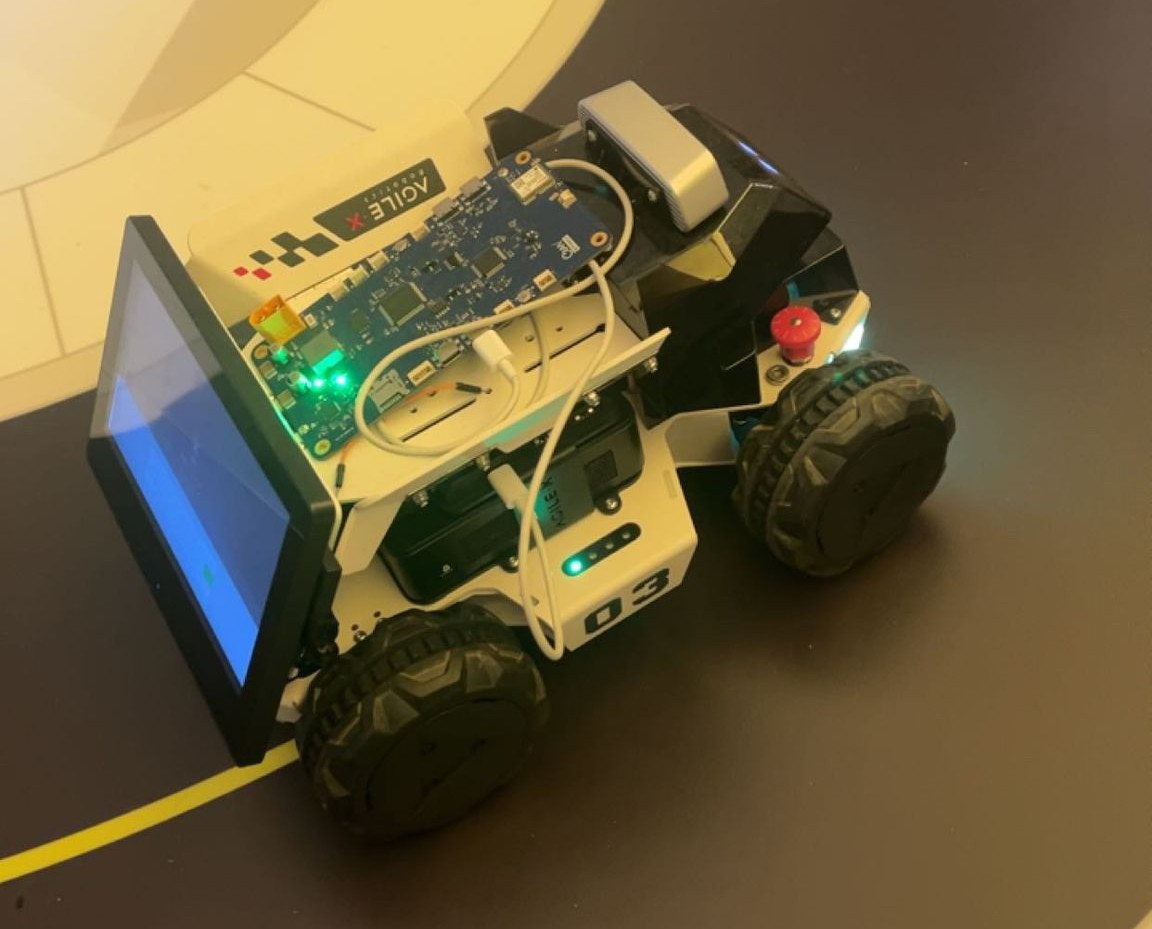
\includegraphics[width=\linewidth,height=\paperheight]{1car_board_smaller_img.jpeg}
    \end{column}
  \end{columns}
  \note{[Sources]\par
    Project title and authorship: \texttt{\detokenize{manuscript_v7_submit.tex}}.\par
    SEGULA visual style and white logo: user-provided \texttt{\detokenize{Official presentation slides_Without page number (ENG) (1).pptx}}.\par
    CRAN logo and vehicle image: user-provided project assets \texttt{\detokenize{assets/R.png}} and \texttt{\detokenize{assets/1car_board_smaller_img.jpeg}}.}
\end{frame}

% -----------------------------------------------------------------------------
\begin{frame}{Why cooperative driving needs a trust boundary}
  \begin{columns}[T,onlytextwidth]
    \begin{column}{0.47\textwidth}
      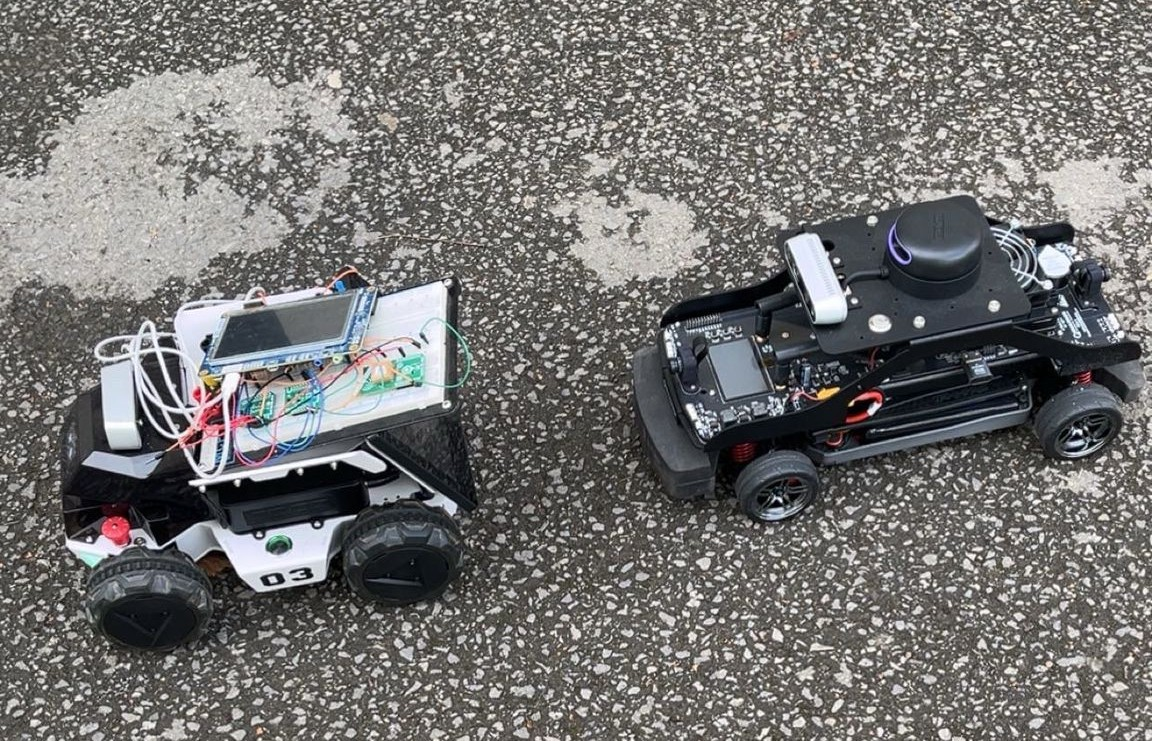
\includegraphics[width=\linewidth,height=0.48\textheight,keepaspectratio]{2car_board_prototype.jpeg}\par
      \vspace{0.05cm}
      {\color{Muted}\fontsize{7.4}{8.9}\selectfont Physical V2V test vehicles with different onboard platforms}
    \end{column}
    \begin{column}{0.48\textwidth}
      \eyebrow{The operating tension}
      {\color{Good}\fontsize{12.5}{14.5}\selectfont\bfseries Cooperation adds useful preview}\par
      \vspace{0.08cm}
      {\fontsize{9.5}{11.4}\selectfont Neighbor position, speed and acceleration support coordinated platooning beyond local sensing alone.}\par
      \vspace{0.20cm}
      {\color{Warn}\fontsize{12.5}{14.5}\selectfont\bfseries Plausible data can still be harmful}\par
      \vspace{0.08cm}
      {\fontsize{9.5}{11.4}\selectfont False, replayed, delayed or missing packets can corrupt a fleet estimate before a conventional controller reacts.}\par
      \vspace{0.18cm}
      {\color{BrandBlue}\rule{0.08cm}{0.67cm}}\hspace{0.13cm}%
      \begin{minipage}[b]{0.86\linewidth}
        {\fontsize{9.2}{11}\selectfont\bfseries Keep cooperation, but reduce dependence on evidence that becomes unreliable.}
      \end{minipage}
    \end{column}
  \end{columns}
  \sourcefoot{Final trust-observer manuscript, introduction and threat model}
  \note{[Sources]\par
    \texttt{\detokenize{ch5/TRust_final/manuscript_v7_submit.tex}}, Introduction and Problem formulation and threat model.\par
    Image: user-provided project asset \texttt{\detokenize{assets/2car_board_prototype.jpeg}}.}
\end{frame}

% -----------------------------------------------------------------------------
\begin{frame}{The trust layer sits between V2V data and the vehicle ECU}
  \eyebrow{Project concept}
  \centering
  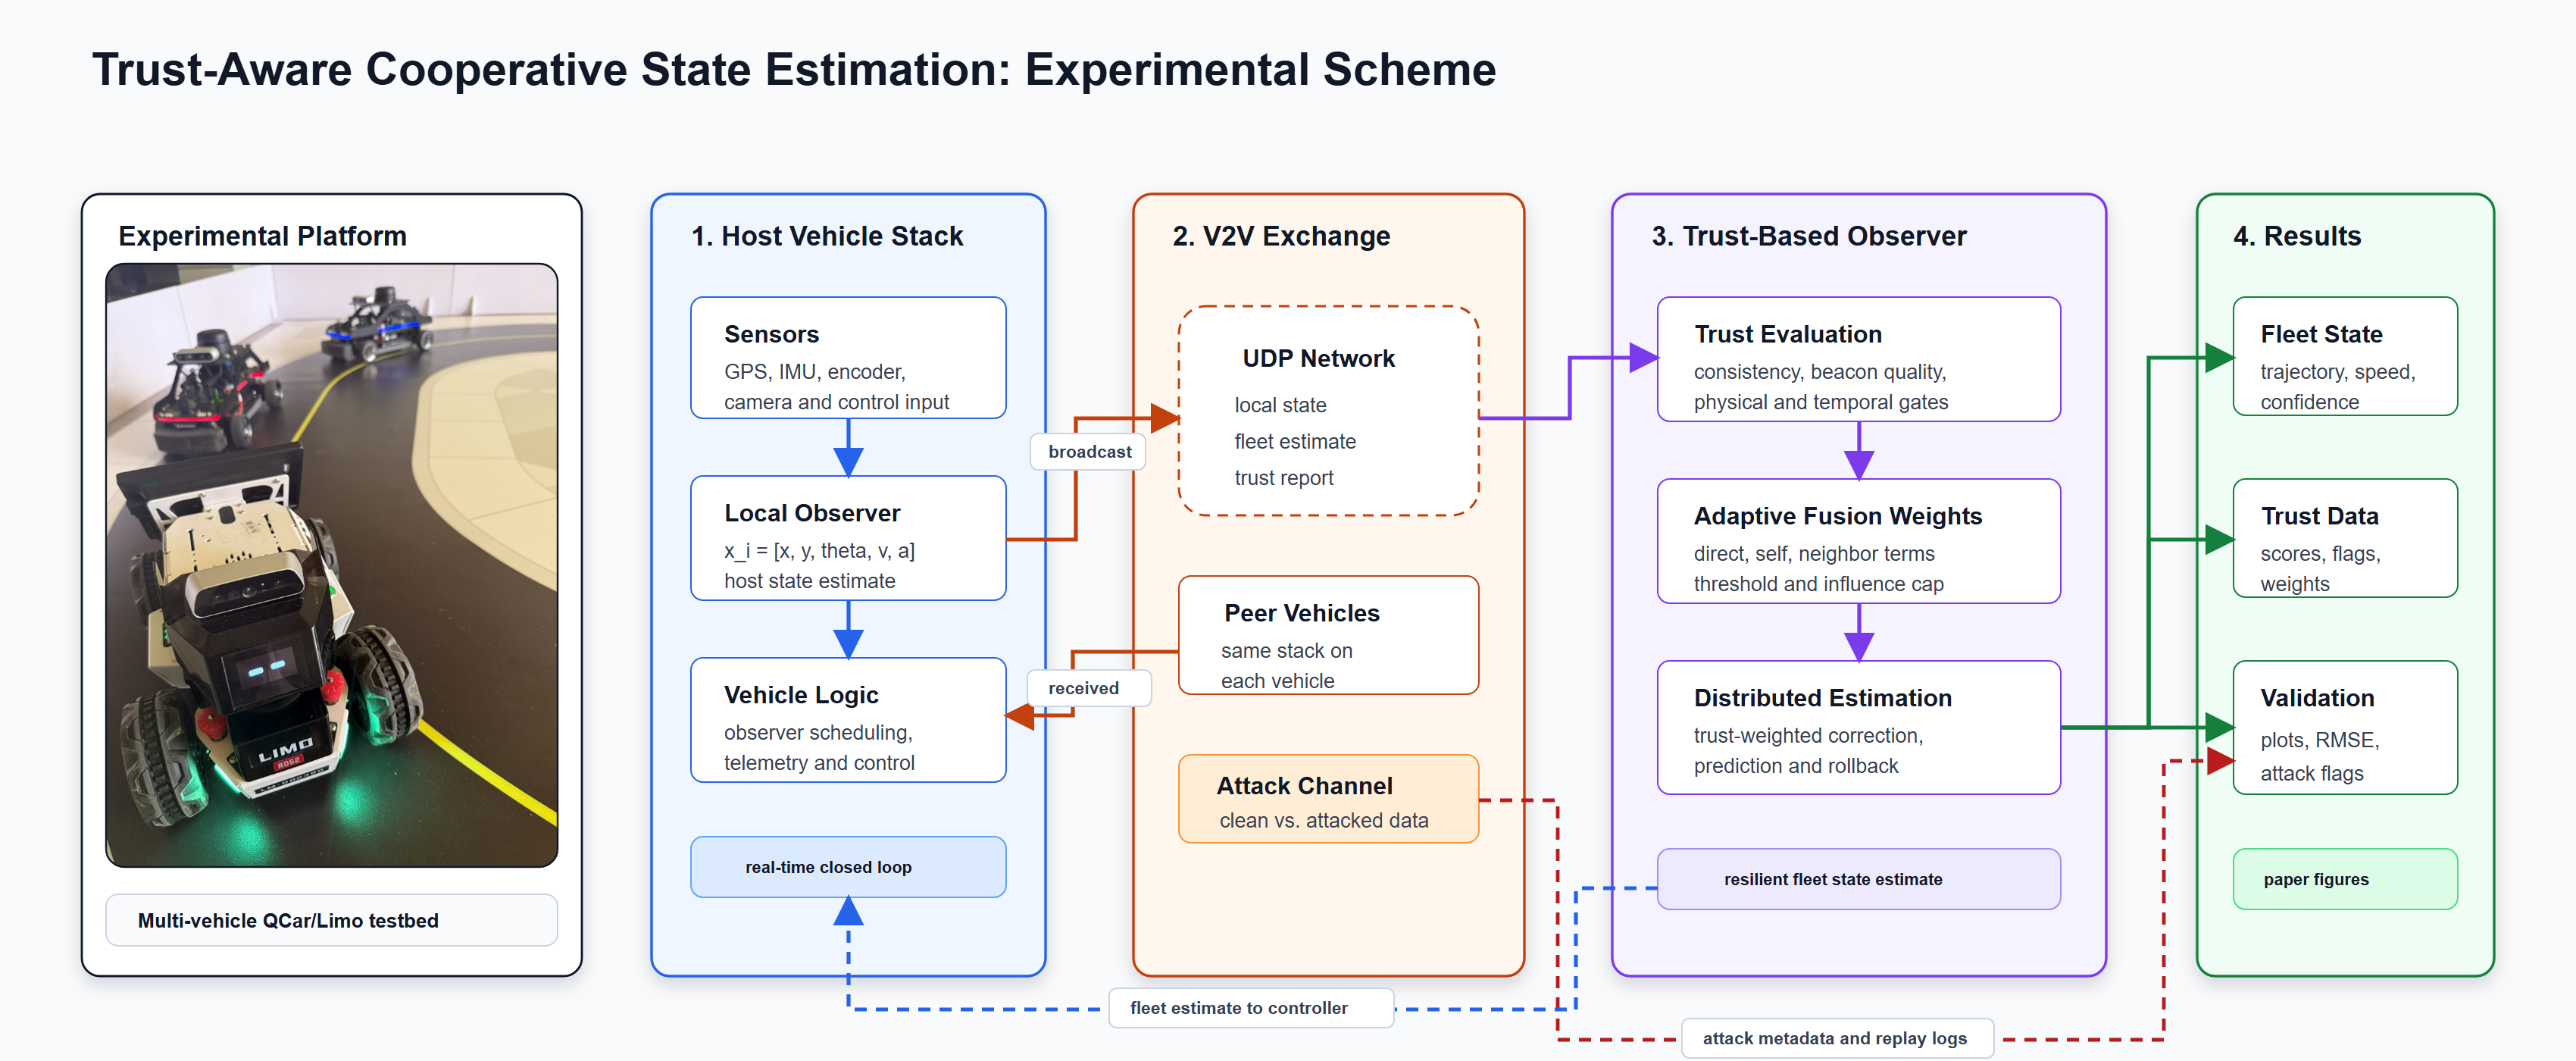
\includegraphics[width=0.98\textwidth,height=0.50\textheight,keepaspectratio]{experimental_scheme.png}
  \vspace{0.05cm}

  \raggedright
  {\color{BrandBlue}\rule{0.08cm}{0.50cm}}\hspace{0.13cm}%
  {\fontsize{8.8}{10.6}\selectfont\bfseries Incoming evidence is screened, weighted and corrected before it reaches the existing vehicle logic.}
  \sourcefoot{Final trust-observer manuscript and project experimental-scheme figure}
  \note{[Sources]\par
    \texttt{\detokenize{ch5/TRust_final/manuscript_v7_submit.tex}}, QCar/LIMO platform and communication stack.\par
    Image: user-provided project asset \texttt{\detokenize{assets/experimental_scheme.png}}.}
\end{frame}

% -----------------------------------------------------------------------------
\begin{frame}{System boundary: the vehicle ECU keeps control}
  \eyebrow{Electronic board integration}
  \vspace{0.04cm}
  \begin{columns}[T,onlytextwidth]
    \begin{column}{0.29\textwidth}
      {\color{BrandCyan}\rule{\linewidth}{0.09cm}}\par
      \vspace{0.12cm}
      {\color{BrandBlue}\fontsize{12.5}{14.5}\selectfont\bfseries Inputs}\par
      \vspace{0.14cm}
      {\fontsize{9.1}{10.9}\selectfont
      \begin{itemize}
        \item IMU and local kinematics
        \item GNSS position and 1PPS timing
        \item Vehicle-bus data and V2V packets
      \end{itemize}}
    \end{column}
    \begin{column}{0.055\textwidth}
      \vspace{1.28cm}\centering{\color{Rule}\fontsize{23}{25}\selectfont$\rightarrow$}
    \end{column}
    \begin{column}{0.31\textwidth}
      {\color{BrandMagenta}\rule{\linewidth}{0.09cm}}\par
      \vspace{0.12cm}
      {\color{BrandMagenta}\fontsize{12.5}{14.5}\selectfont\bfseries Trust edge module}\par
      \vspace{0.14cm}
      {\fontsize{9.1}{10.9}\selectfont
      \begin{itemize}
        \item Timing and packet-validity gates
        \item State estimation and source weighting
        \item Rollback, re-anchoring and audit logs
      \end{itemize}}
    \end{column}
    \begin{column}{0.055\textwidth}
      \vspace{1.28cm}\centering{\color{Rule}\fontsize{23}{25}\selectfont$\rightarrow$}
    \end{column}
    \begin{column}{0.29\textwidth}
      {\color{Good}\rule{\linewidth}{0.09cm}}\par
      \vspace{0.12cm}
      {\color{Good}\fontsize{12.5}{14.5}\selectfont\bfseries Outputs}\par
      \vspace{0.14cm}
      {\fontsize{9.1}{10.9}\selectfont
      \begin{itemize}
        \item Trusted state estimates
        \item Attack, trust and health flags
        \item Safe-mode request through a gateway
      \end{itemize}}
    \end{column}
  \end{columns}
  \vspace{0.18cm}
  {\color{BrandBlue}\fontsize{9.2}{11}\selectfont\bfseries Planned path:}\hspace{0.08cm}%
  {\fontsize{9.2}{11}\selectfont monitor first; the ACC/CACC ECU retains acceleration and braking authority.}
  \sourcefoot{Thesis Chapter 6, board requirements and integration roadmap}
  \note{[Sources]\par
    \texttt{\detokenize{ch6/ch6_main.tex}}, Custom embedded electronic board for future onboard deployment, component selection, firmware structure and integration roadmap.}
\end{frame}

% -----------------------------------------------------------------------------
\begin{frame}{Response to an unreliable packet}
  \eyebrow{One progressive response chain}
  \vspace{0.04cm}
  \begin{columns}[T,onlytextwidth]
    \begin{column}{0.18\textwidth}
      {\color{Good}\rule{\linewidth}{0.10cm}}\par\vspace{0.08cm}
      {\color{Good}\fontsize{16}{18}\selectfont\bfseries 01}\par
      {\fontsize{9.4}{11.2}\selectfont\bfseries ACCEPT}\par
      {\color{Muted}\fontsize{7.3}{8.8}\selectfont Evidence is fresh and consistent.}
    \end{column}
    \begin{column}{0.18\textwidth}
      {\color{BrandCyan}\rule{\linewidth}{0.10cm}}\par\vspace{0.08cm}
      {\color{BrandCyan}\fontsize{16}{18}\selectfont\bfseries 02}\par
      {\fontsize{9.4}{11.2}\selectfont\bfseries DOWN-WEIGHT}\par
      {\color{Muted}\fontsize{7.3}{8.8}\selectfont Reduce the source's influence.}
    \end{column}
    \begin{column}{0.18\textwidth}
      {\color{Warn}\rule{\linewidth}{0.10cm}}\par\vspace{0.08cm}
      {\color{Warn}\fontsize{16}{18}\selectfont\bfseries 03}\par
      {\fontsize{9.4}{11.2}\selectfont\bfseries ISOLATE}\par
      {\color{Muted}\fontsize{7.3}{8.8}\selectfont Set the source weight to zero.}
    \end{column}
    \begin{column}{0.18\textwidth}
      {\color{Purple}\rule{\linewidth}{0.10cm}}\par\vspace{0.08cm}
      {\color{Purple}\fontsize{16}{18}\selectfont\bfseries 04}\par
      {\fontsize{9.4}{11.2}\selectfont\bfseries CORRECT}\par
      {\color{Muted}\fontsize{7.3}{8.8}\selectfont Roll back and re-anchor state.}
    \end{column}
    \begin{column}{0.18\textwidth}
      {\color{BrandBlue}\rule{\linewidth}{0.10cm}}\par\vspace{0.08cm}
      {\color{BrandBlue}\fontsize{16}{18}\selectfont\bfseries 05}\par
      {\fontsize{9.4}{11.2}\selectfont\bfseries FALLBACK}\par
      {\color{Muted}\fontsize{7.3}{8.8}\selectfont Request local-control mode.}
    \end{column}
  \end{columns}
  \vspace{0.24cm}
  \begin{columns}[T,onlytextwidth]
    \begin{column}{0.31\textwidth}
      {\color{BrandCyan}\rule{\linewidth}{0.06cm}}\par\vspace{0.05cm}
      {\fontsize{8.4}{10}\selectfont\bfseries Prevent new contamination}\par
      {\color{Muted}\fontsize{7.3}{8.8}\selectfont Packet gate, down-weighting and isolation.}
    \end{column}
    \begin{column}{0.31\textwidth}
      {\color{BrandMagenta}\rule{\linewidth}{0.06cm}}\par\vspace{0.05cm}
      {\fontsize{8.4}{10}\selectfont\bfseries Repair recent history}\par
      {\color{Muted}\fontsize{7.3}{8.8}\selectfont Rollback and anchoring remove stored error.}
    \end{column}
    \begin{column}{0.31\textwidth}
      {\color{BrandBlue}\rule{\linewidth}{0.06cm}}\par\vspace{0.05cm}
      {\fontsize{8.4}{10}\selectfont\bfseries Protect vehicle control}\par
      {\color{Muted}\fontsize{7.3}{8.8}\selectfont Degrade only when confidence is insufficient.}
    \end{column}
  \end{columns}
  \vspace{0.12cm}
  {\color{Warn}\fontsize{8.5}{10.2}\selectfont\bfseries Current scope:}\hspace{0.06cm}%
  {\fontsize{8.5}{10.2}\selectfont no direct actuator override; the existing vehicle controller keeps command authority.}
  \sourcefoot{Final manuscript packet gate, rollback and trust-gated ACC/CACC}
  \note{[Sources]\par
    \texttt{\detokenize{ch5/TRust_final/manuscript_v7_submit.tex}}, packet validity gate, Contamination rollback, and Distributed state estimation for platoon control.\par
    \texttt{\detokenize{ch6/ch6_main.tex}}, integration roadmap and safe degradation modes.}
\end{frame}

% -----------------------------------------------------------------------------
\begin{frame}{Validation progressed from simulation to embedded hardware}
  \begin{columns}[T,onlytextwidth]
    \begin{column}{0.51\textwidth}
      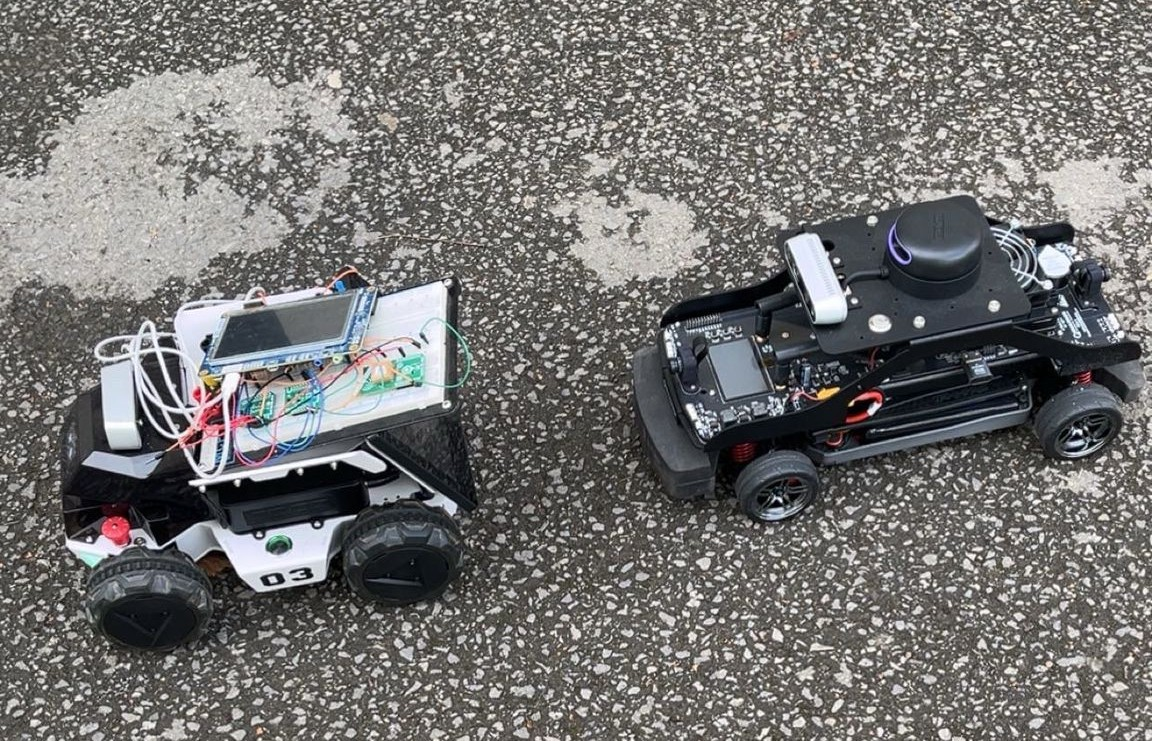
\includegraphics[width=\linewidth,height=0.47\textheight,keepaspectratio]{2car_board_prototype.jpeg}\par
      \vspace{0.05cm}
      {\color{Muted}\fontsize{7.4}{8.9}\selectfont Multi-platform physical test setup}
    \end{column}
    \begin{column}{0.44\textwidth}
      \eyebrow{Three validation levels}
      \stepnumber{01}\hspace{0.16cm}{\fontsize{11.3}{13.4}\selectfont\bfseries Numerical campaign}\par
      {\color{Muted}\fontsize{8.3}{10}\selectfont Five vehicles, controlled ground truth and repeated channel attacks.}\par
      \vspace{0.17cm}
      \stepnumber{02}\hspace{0.16cm}{\fontsize{11.3}{13.4}\selectfont\bfseries Digital and physical loop}\par
      {\color{Muted}\fontsize{8.3}{10}\selectfont QLabs plus QCar/LIMO packet exchange, timing and closed-loop trajectories.}\par
      \vspace{0.17cm}
      \stepnumber{03}\hspace{0.16cm}{\fontsize{11.3}{13.4}\selectfont\bfseries Embedded transfer}\par
      {\color{Muted}\fontsize{8.3}{10}\selectfont Four-layer PCB, RTOS scheduling, sensing, radio communication and logging.}\par
    \end{column}
  \end{columns}
  \sourcefoot{Thesis Chapter 6 methodology and final manuscript validation layers}
  \note{[Sources]\par
    \texttt{\detokenize{ch6/ch6_main.tex}}, Experimental methodology: from virtual validation to real trials.\par
    \texttt{\detokenize{ch5/TRust_final/manuscript_v7_submit.tex}}, aggregate attack-window performance.\par
    Image: user-provided project asset \texttt{\detokenize{assets/2car_board_prototype.jpeg}}.}
\end{frame}

% -----------------------------------------------------------------------------
\begin{frame}{The trust logic suppresses corrupted sources in the tested campaign}
  \eyebrow{Core method - trust-aware distributed estimation}
  {\fontsize{12}{14.3}\selectfont\bfseries Reliability becomes an online fusion weight instead of a fixed assumption.}\par
  \begin{columns}[T,onlytextwidth]
    \begin{column}{0.28\textwidth}
      \metric{100\%}{Detection across the tested attacks and channel configurations}
    \end{column}
    \begin{column}{0.31\textwidth}
      \metric{80.64--98.44\%}{Attacked-source zero rate during the attack window}
    \end{column}
    \begin{column}{0.31\textwidth}
      \metric{28--88 ms}{Mean threshold-crossing delay after the 10 s attack onset}
    \end{column}
  \end{columns}
  \vspace{0.10cm}
  \centering
  {\fontsize{7.8}{9.4}\selectfont
  \renewcommand{\arraystretch}{1.08}
  \begin{tabular}{lccc}
    \toprule
    \textbf{Corrupted channel} & \textbf{Mean combined RMSE} & \textbf{Trust drop} & \textbf{Source zero rate} \\
    \midrule
    Local & 0.643 & 0.319 & 80.64\% \\
    Global & 0.393 & 0.460 & 92.90\% \\
    Local + global & 0.567 & 0.544 & 98.44\% \\
    \bottomrule
  \end{tabular}}
  \sourcefoot{Final trust-observer manuscript, aggregate attack-window performance}
  \note{[Sources]\par
    \texttt{\detokenize{ch5/TRust_final/manuscript_v7_submit.tex}}, Numerical simulation results, aggregate attack-window performance table.\par
    Detection delay is calculated from reported mean threshold times minus the 10 s attack onset.}
\end{frame}

% -----------------------------------------------------------------------------
\begin{frame}{Rollback removes contamination already stored in the state}
  \eyebrow{Delayed-decision recovery}
  \begin{columns}[T,onlytextwidth]
    \begin{column}{0.65\textwidth}
      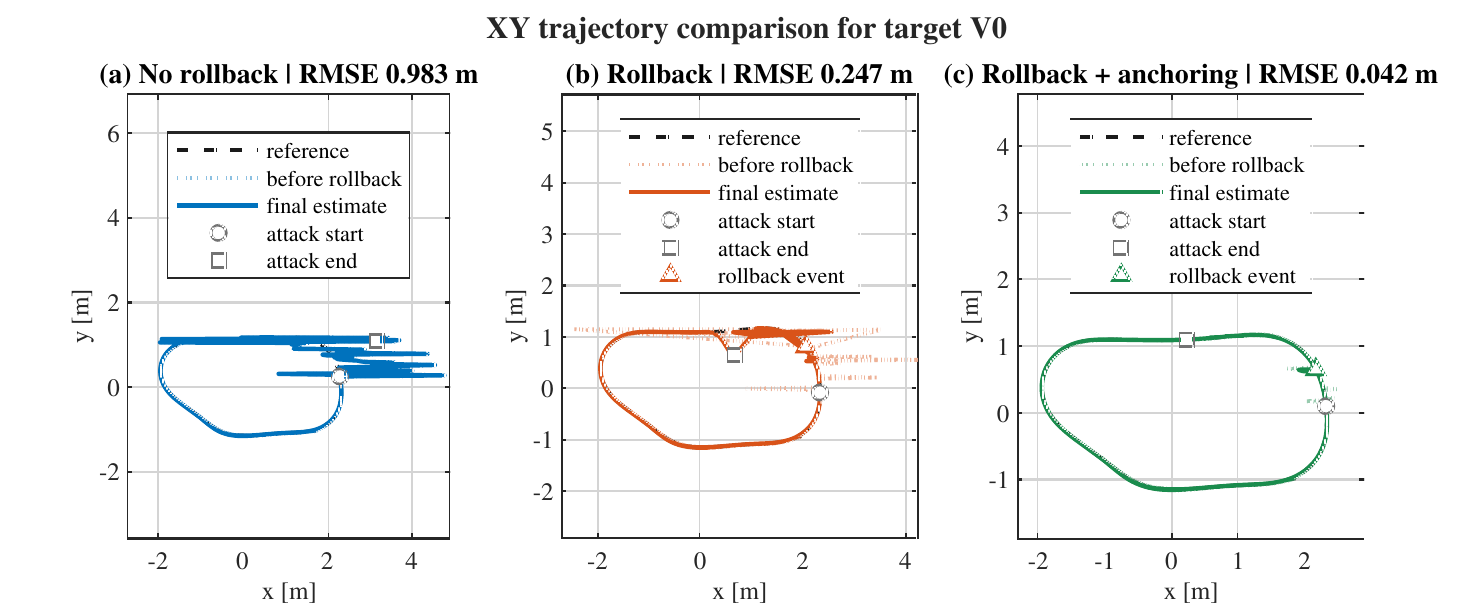
\includegraphics[width=\linewidth,height=0.59\textheight,keepaspectratio]{xy_case2_local.png}
    \end{column}
    \begin{column}{0.30\textwidth}
      \vspace{0.08cm}
      \quietmetric{0.983 m}{No rollback}\par
      \vspace{0.23cm}
      \quietmetric{0.247 m}{Rollback}\par
      \vspace{0.23cm}
      {\color{BrandCyan}\fontsize{20}{22}\selectfont\bfseries 0.042 m}\par
      {\color{Muted}\fontsize{8.4}{10.1}\selectfont Rollback plus accepted relative-pose anchoring}\par
      \vspace{0.20cm}
      {\color{BrandBlue}\fontsize{8.2}{9.8}\selectfont\bfseries Local-channel Case 2 RMSE}
    \end{column}
  \end{columns}
  \sourcefoot{Final manuscript QCar/LIMO rollback and anchoring results}
  \note{[Sources]\par
    \texttt{\detokenize{ch5/TRust_final/manuscript_v7_submit.tex}}, Rollback and anchoring results and Closed-loop trajectory diagnostics.\par
    Image converted from \texttt{\detokenize{ch5/TRust_final/img/XY_case2_local.eps}}.}
\end{frame}

% -----------------------------------------------------------------------------
\begin{frame}{Trust supports a controlled move from CACC toward local ACC}
  \eyebrow{Control application - trust-gated ACC/CACC}
  \begin{columns}[T,onlytextwidth]
    \begin{column}{0.59\textwidth}
      \centering
      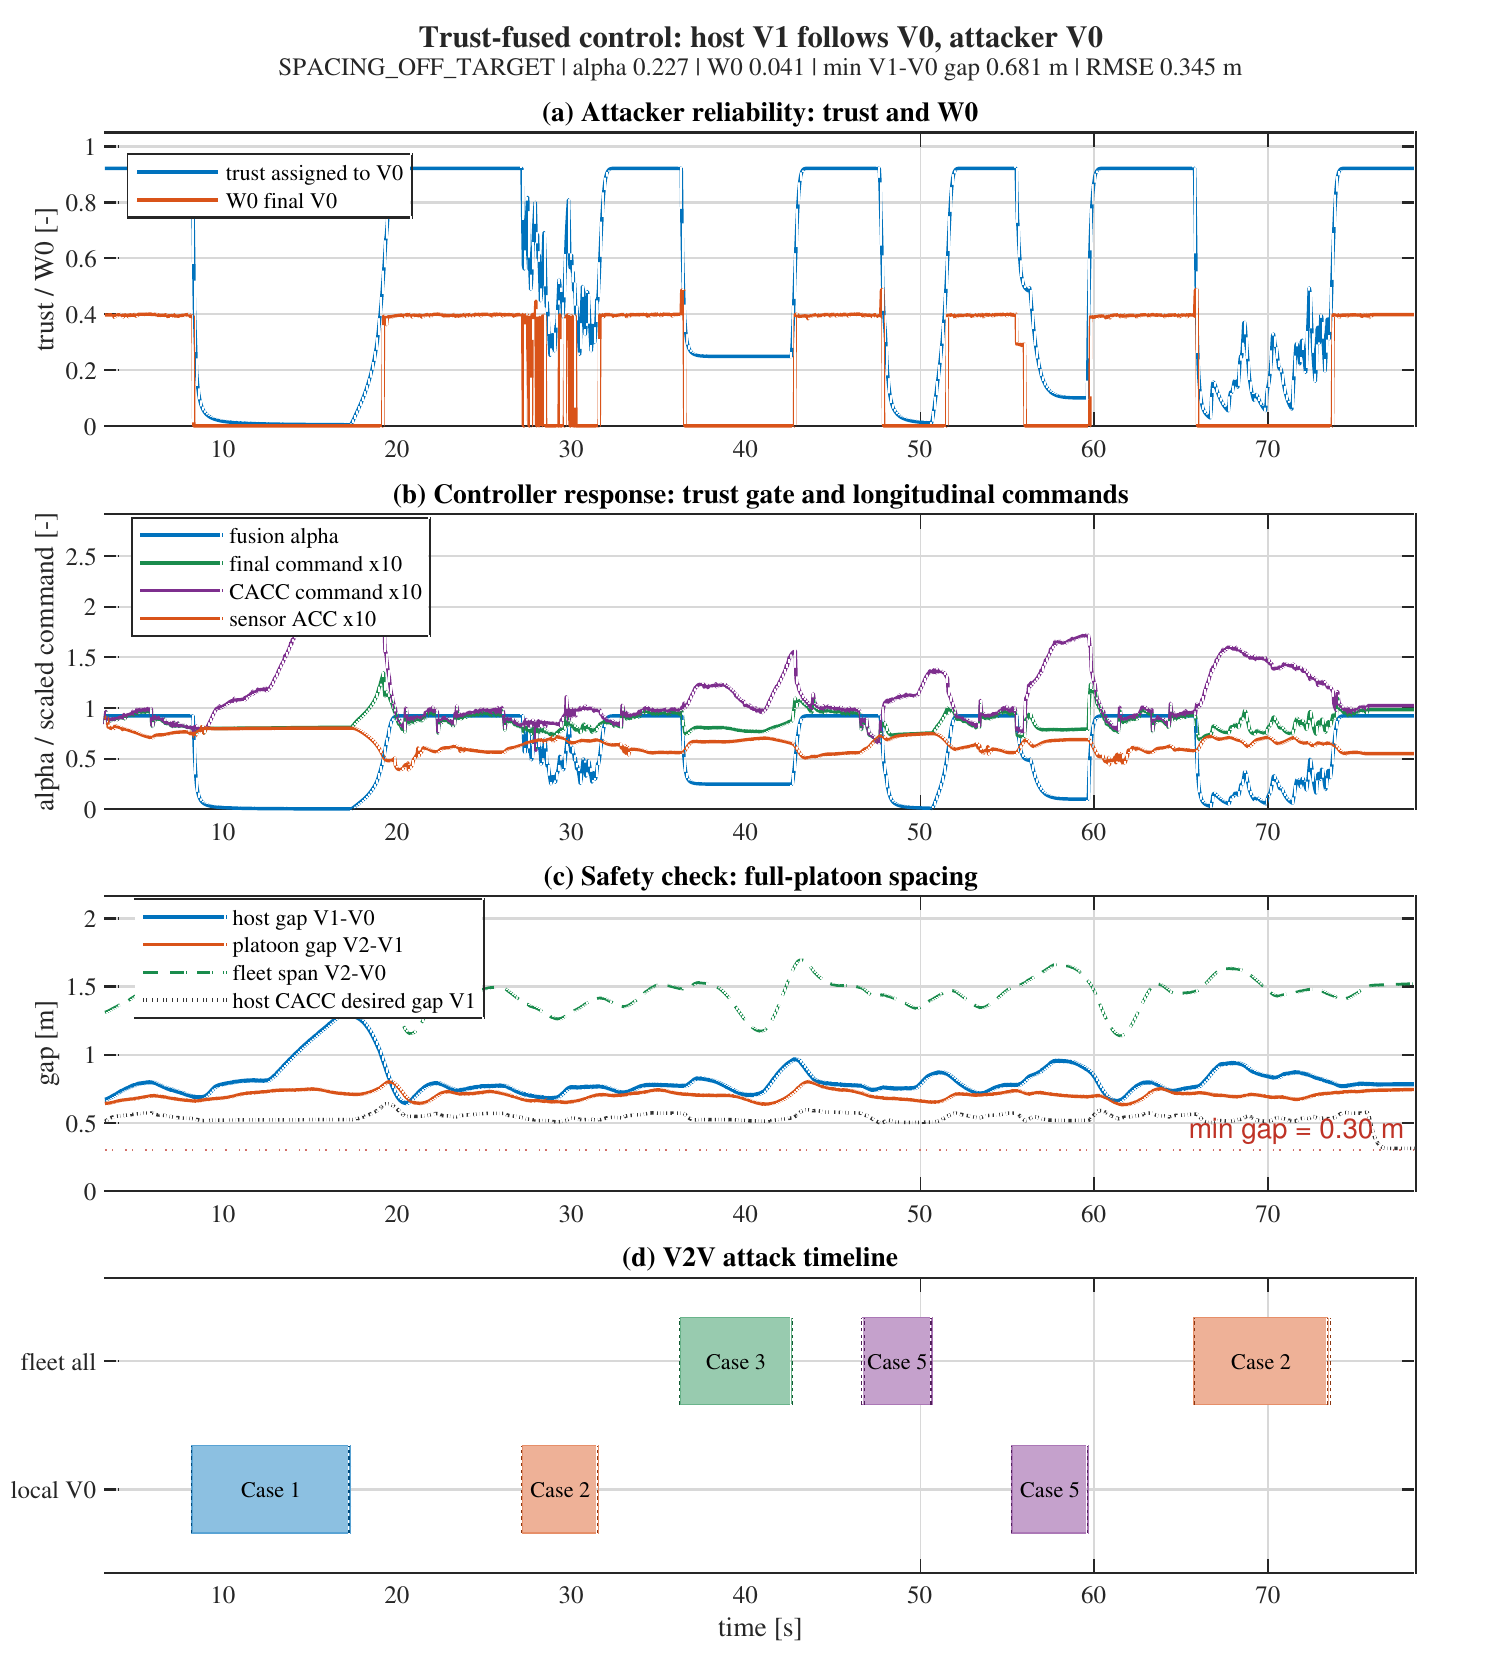
\includegraphics[height=0.53\textheight,width=\linewidth,keepaspectratio]{controller_fusion.png}
    \end{column}
    \begin{column}{0.36\textwidth}
      \quietmetric{$<0.05$}{Mean attacked-source observer weight}\par
      \vspace{0.22cm}
      \quietmetric{0.681 m}{V1 minimum path-projected gap}\par
      \vspace{0.22cm}
      \quietmetric{0.637 m}{V2 minimum path-projected gap}\par
      \vspace{0.16cm}
      {\color{Warn}\fontsize{7.8}{9.4}\selectfont\bfseries Scope:}\hspace{0.05cm}%
      {\fontsize{7.8}{9.4}\selectfont both gaps exceed the 0.30 m study margin; this is a feasibility result, not a collision guarantee.}
    \end{column}
  \end{columns}
  \sourcefoot{Final trust-observer manuscript, trust-gated ACC/CACC metrics}
  \note{[Sources]\par
    \texttt{\detokenize{ch5/TRust_final/manuscript_v7_submit.tex}}, Distributed state estimation for platoon control and attack-window closed-loop metrics.\par
    Image converted from \texttt{\detokenize{ch5/TRust_final/img/controller_fusion.eps}}.}
\end{frame}

% -----------------------------------------------------------------------------
\begin{frame}{The same operating loop is reproduced virtually and physically}
  \begin{columns}[T,onlytextwidth]
    \begin{column}{0.62\textwidth}
      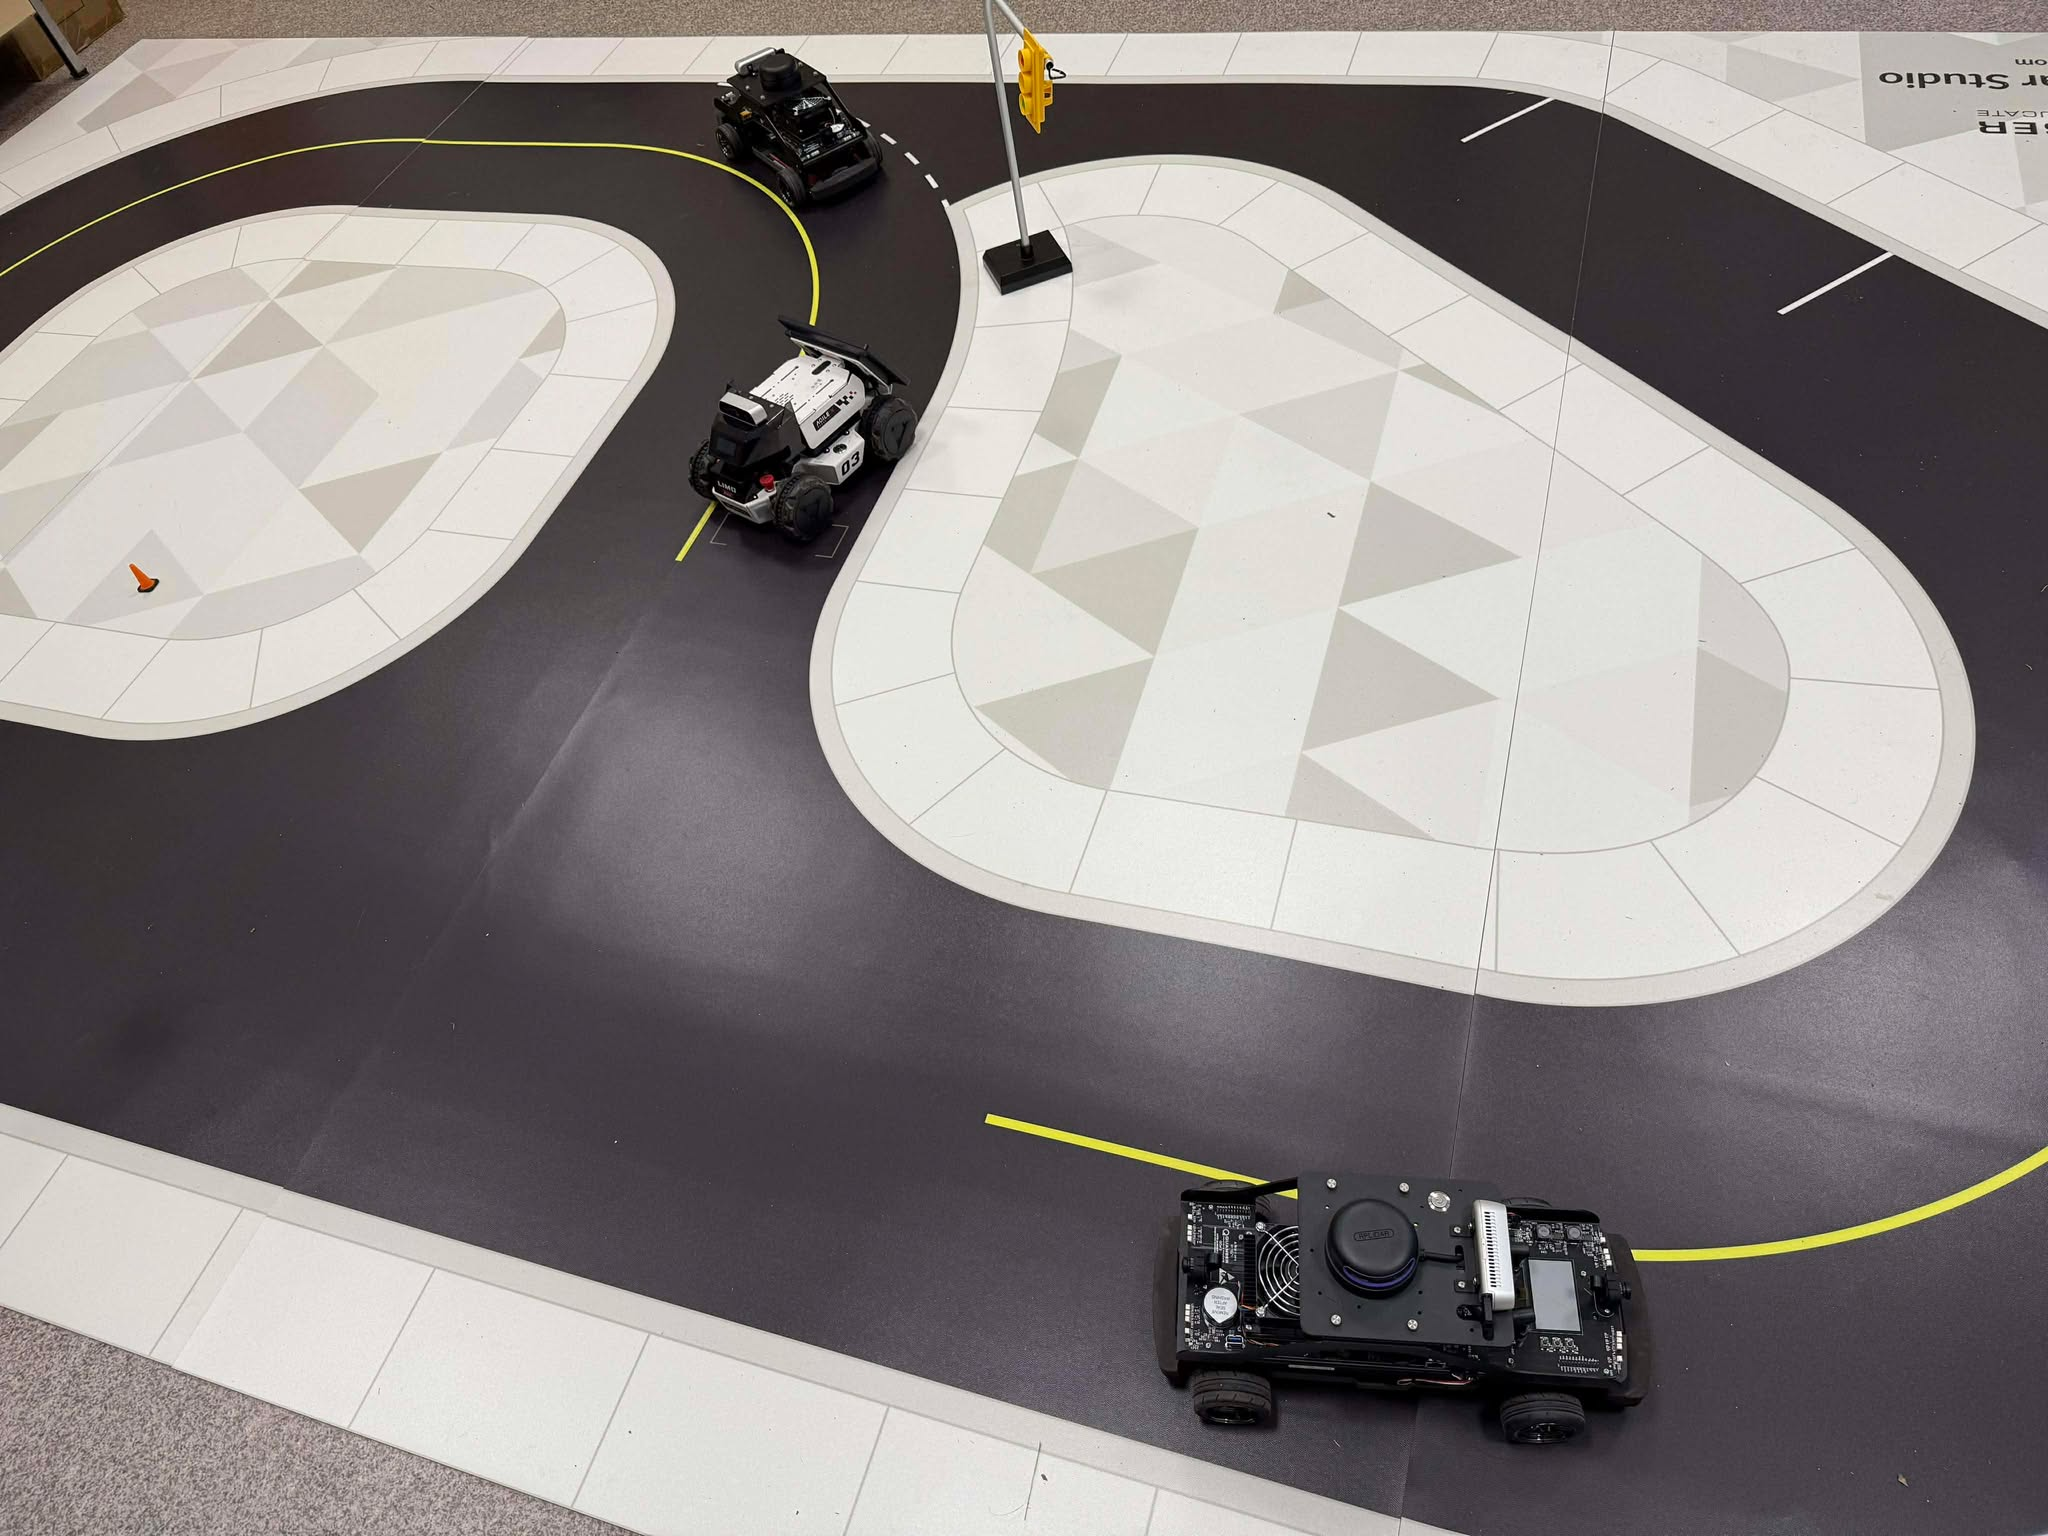
\includegraphics[width=\linewidth,height=0.44\textheight,keepaspectratio]{scale_model_track.jpg}\par
      \vspace{0.05cm}
      {\color{BrandBlue}\fontsize{8.4}{10.1}\selectfont\bfseries Physical QCar/LIMO track}\par
      {\color{Muted}\fontsize{7.6}{9.1}\selectfont Real packet timing, sensor noise, scheduling and actuator response.}
    \end{column}
    \begin{column}{0.33\textwidth}
      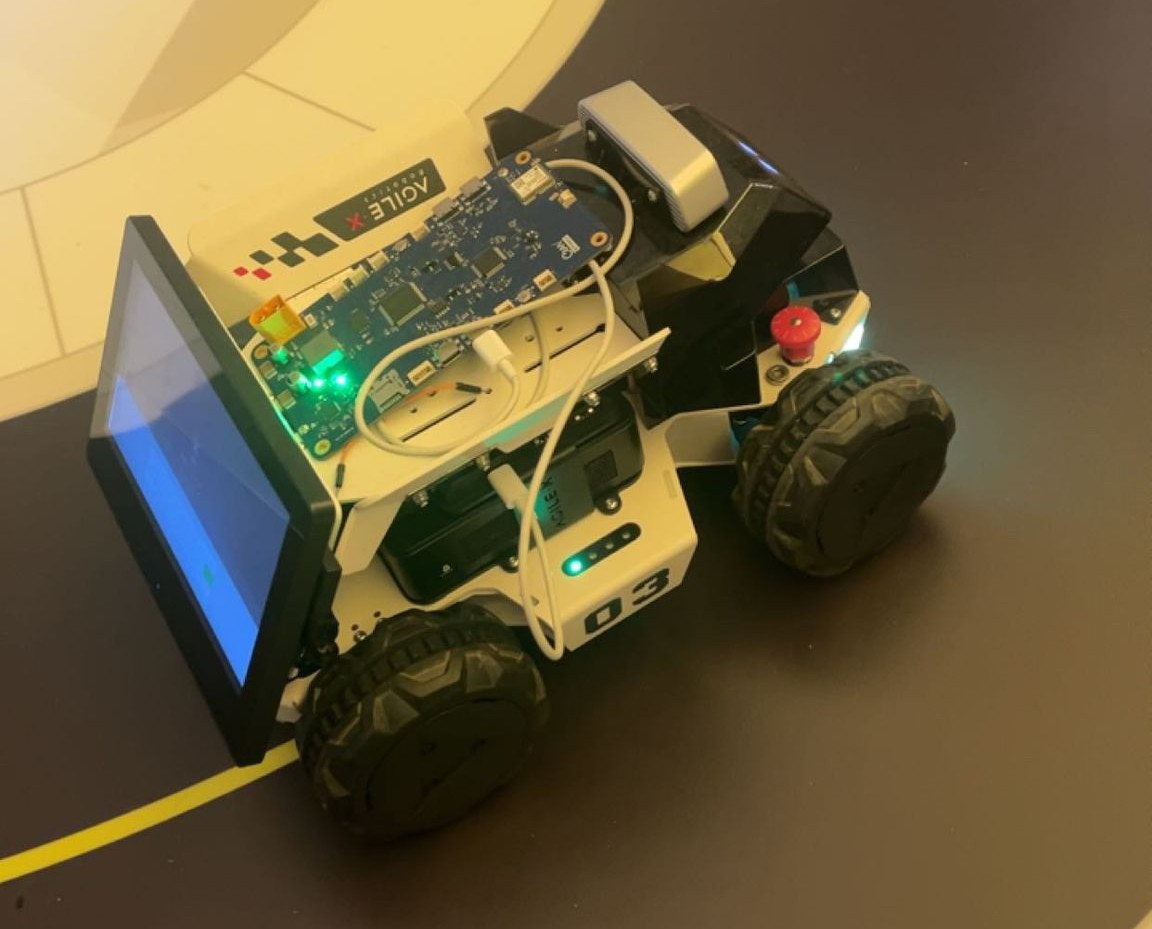
\includegraphics[width=0.92\linewidth]{1car_board_smaller_img.jpeg}\par
      \vspace{0.05cm}
      {\color{BrandBlue}\fontsize{8.4}{10.1}\selectfont\bfseries Research PCB on the vehicle}\par
      {\color{Muted}\fontsize{7.6}{9.1}\selectfont
        \textbf{Physical loop:} embedded timing, sensing and communication.\par
        \textbf{Virtual twin:} the same states and attacks are repeated in QLabs.}
    \end{column}
  \end{columns}
  \sourcefoot{Thesis Chapter 6 and final manuscript QCar/LIMO implementation}
  \note{[Sources]\par
    Images: user-provided project assets \texttt{\detokenize{assets/scale_model_track.jpg}}, \texttt{\detokenize{assets/1car_board_smaller.jpeg}} and \texttt{\detokenize{assets/qlabs_map.png}}.\par
    \texttt{\detokenize{ch6/ch6_main.tex}}, QLabs environment and experimental workflow.\par
    \texttt{\detokenize{ch5/TRust_final/manuscript_v7_submit.tex}}, QCar/LIMO platform validation.}
\end{frame}

% -----------------------------------------------------------------------------
\begin{frame}{Prototype evolution: breadboard to four-layer PCB}
  \eyebrow{Embedded transfer}
  \begin{columns}[T,onlytextwidth]
    \begin{column}{0.31\textwidth}
      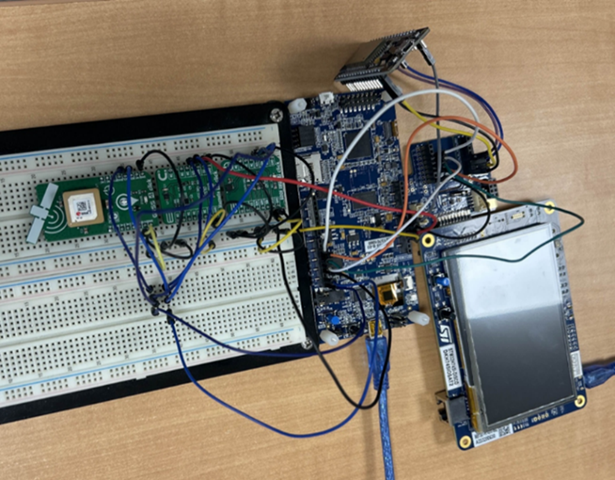
\includegraphics[width=\linewidth,height=0.21\textheight,keepaspectratio]{development_bringup.png}\par
      \vspace{0.08cm}
      \stepnumber{01}\hspace{0.10cm}{\fontsize{10.7}{12.7}\selectfont\bfseries Bring-up}\par
      {\color{Muted}\fontsize{7.5}{9}\selectfont Sensor, display and communication interfaces validated on the bench.}
    \end{column}
    \begin{column}{0.31\textwidth}
      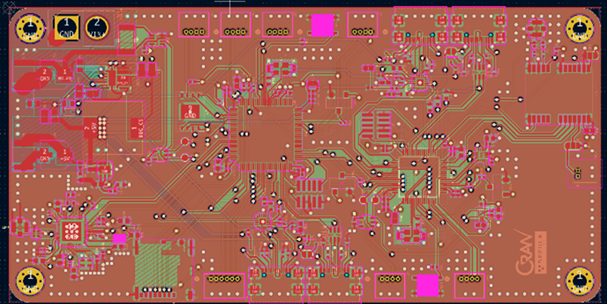
\includegraphics[width=\linewidth,height=0.21\textheight,keepaspectratio]{pcb_layout.png}\par
      \vspace{0.08cm}
      \stepnumber{02}\hspace{0.10cm}{\fontsize{10.7}{12.7}\selectfont\bfseries Layout}\par
      {\color{Muted}\fontsize{7.5}{9}\selectfont Four-layer routing, grounding and power distribution prepared for manufacture.}
    \end{column}
    \begin{column}{0.31\textwidth}
      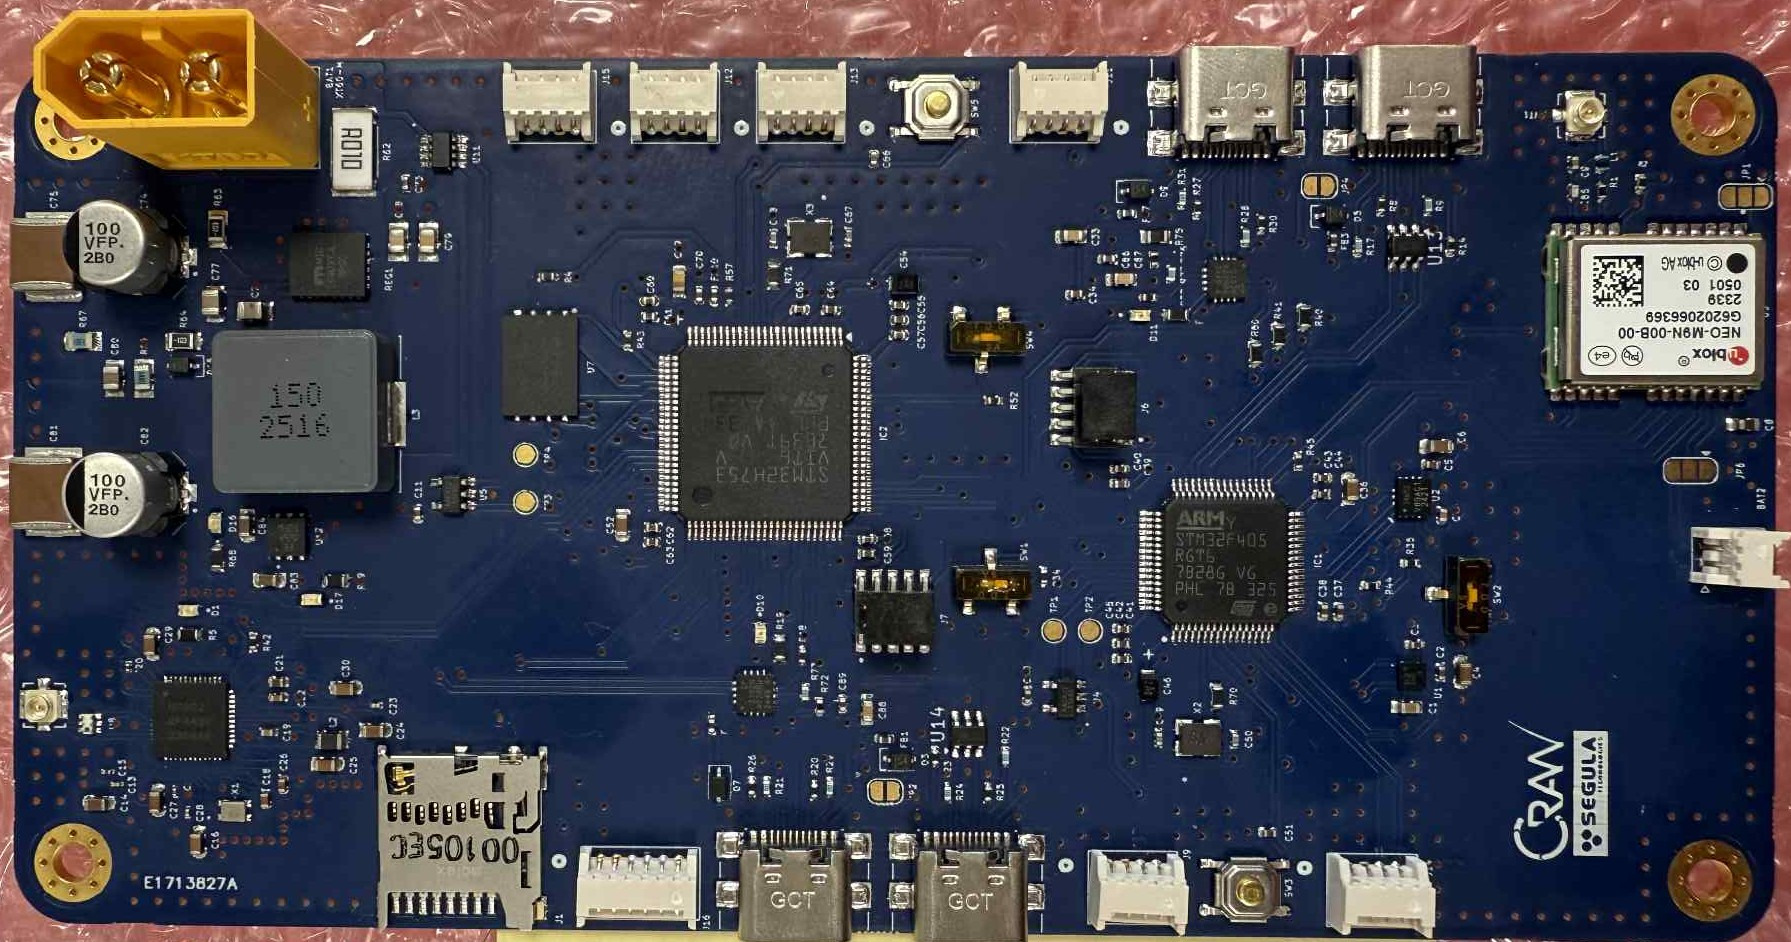
\includegraphics[width=\linewidth,height=0.21\textheight,keepaspectratio]{pcb_photo.jpg}\par
      \vspace{0.08cm}
      \stepnumber{03}\hspace{0.10cm}{\fontsize{10.7}{12.7}\selectfont\bfseries Manufactured board}\par
      {\color{Muted}\fontsize{7.5}{9}\selectfont MCU/RTOS platform with sensing, timing, Wi-Fi, storage and development access.}
    \end{column}
  \end{columns}
  \vspace{0.14cm}
  {\color{BrandBlue}\fontsize{8.1}{9.7}\selectfont\bfseries Bring-up evidence: stable 100 Hz RTOS, UART, GNSS acquisition and functional Wi-Fi 6 tests.}
  \sourcefoot{Thesis Chapter 6, board design and first firmware validation tests}
  \note{[Sources]\par
    Images: user-provided project assets \texttt{\detokenize{assets/development_bringup.png}}, \texttt{\detokenize{assets/pcb_layout.png}} and \texttt{\detokenize{assets/pcb_photo.jpg}}.\par
    \texttt{\detokenize{ch6/ch6_main.tex}}, Architecture and PCB design; Firmware structure and first validation tests.}
\end{frame}

% -----------------------------------------------------------------------------
\begin{frame}{The current PCB is an embedded trust demonstrator}
  \begin{columns}[T,onlytextwidth]
    \begin{column}{0.57\textwidth}
      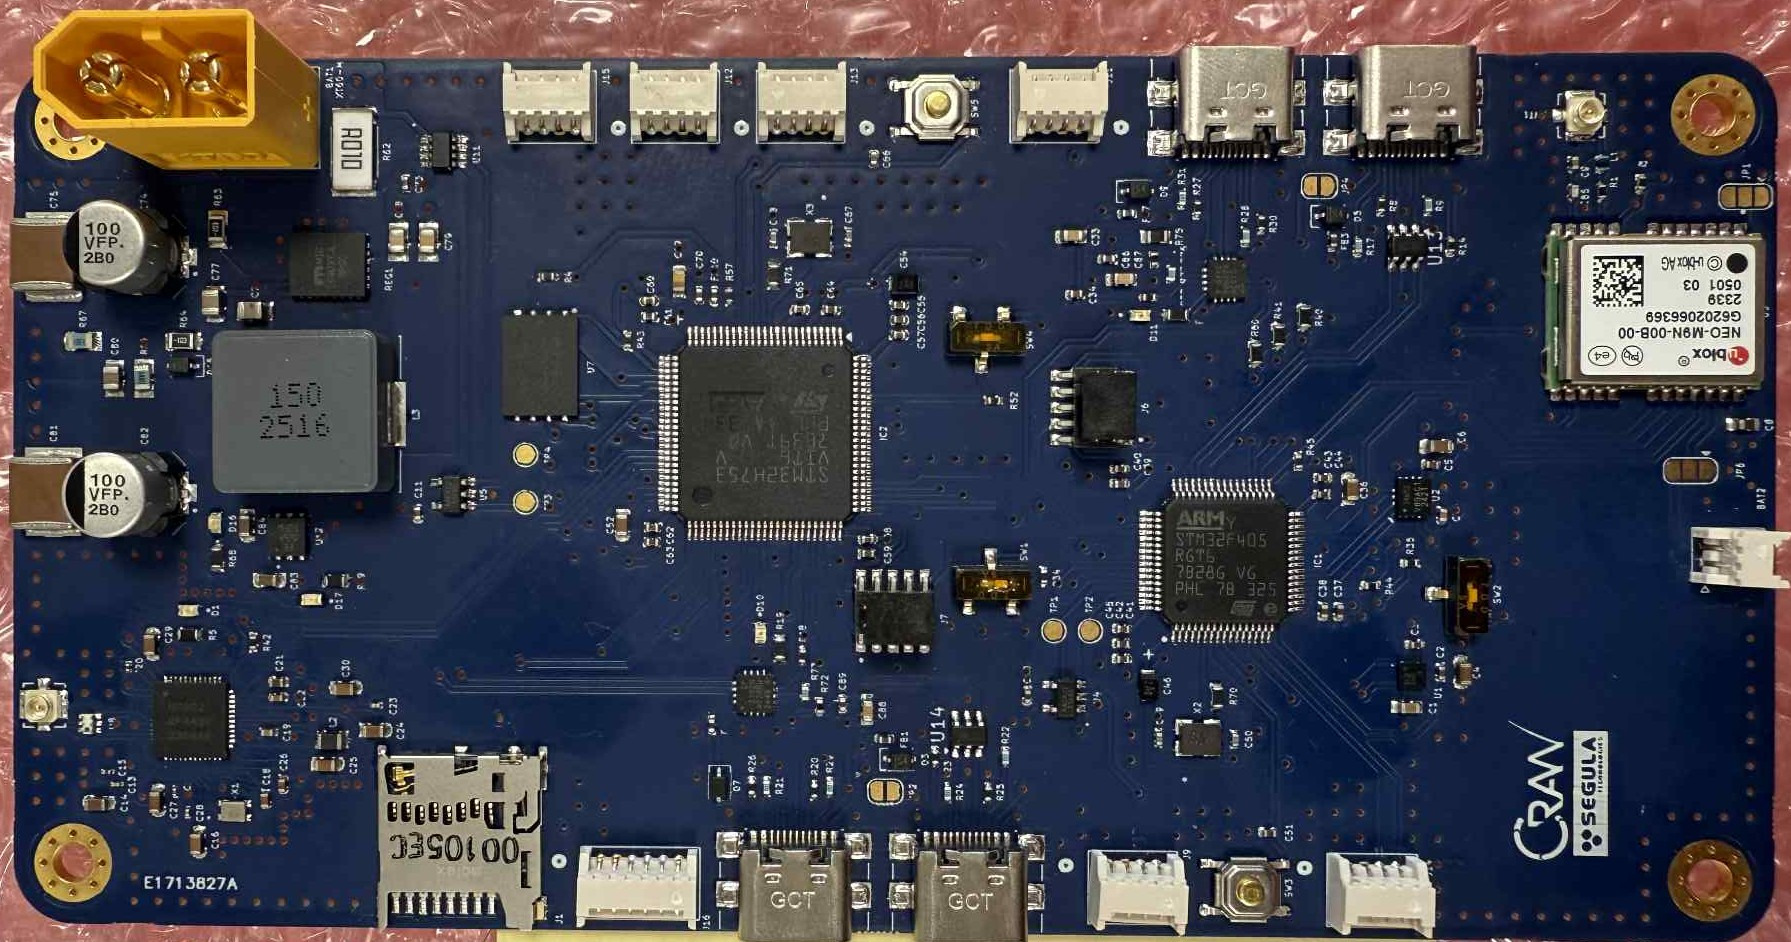
\includegraphics[width=\linewidth,height=0.46\textheight,keepaspectratio]{pcb_photo.jpg}
    \end{column}
    \begin{column}{0.38\textwidth}
      \eyebrow{What it already supports}
      {\color{BrandBlue}\fontsize{10.5}{12.5}\selectfont\bfseries Sensing and timing}\par
      {\fontsize{8}{9.6}\selectfont IMU, GNSS, 1PPS timing and selected vehicle kinematics.}\par
      \vspace{0.12cm}
      {\color{BrandBlue}\fontsize{10.5}{12.5}\selectfont\bfseries Interfaces}\par
      {\fontsize{8}{9.6}\selectfont Research Wi-Fi, UART/USB, storage and synchronized logging.}\par
      \vspace{0.12cm}
      {\color{BrandBlue}\fontsize{10.5}{12.5}\selectfont\bfseries Runtime role}\par
      {\fontsize{8}{9.6}\selectfont State estimation, source trust, rollback and exported health flags.}
    \end{column}
  \end{columns}
  \vspace{0.08cm}
  {\color{Warn}\fontsize{8}{9.6}\selectfont\bfseries Product gaps:}\hspace{0.05cm}%
  {\fontsize{7.8}{9.3}\selectfont protected power, CAN/CAN-FD, production V2X radio, secure key storage, enclosure and qualification.}
  \sourcefoot{Thesis Chapter 6, board requirements, interfaces and qualification roadmap}
  \note{[Sources]\par
    Image: user-provided project asset \texttt{\detokenize{assets/pcb_photo.jpg}}.\par
    \texttt{\detokenize{ch6/ch6_main.tex}}, board motivation, functional requirements, component selection, firmware structure and integration roadmap.}
\end{frame}

% -----------------------------------------------------------------------------
\begin{frame}{Commercial OBUs define the target product envelope}
  \eyebrow{Existing V2V onboard units}
  \begin{columns}[T,onlytextwidth]
    \begin{column}{0.47\textwidth}
      \centering
      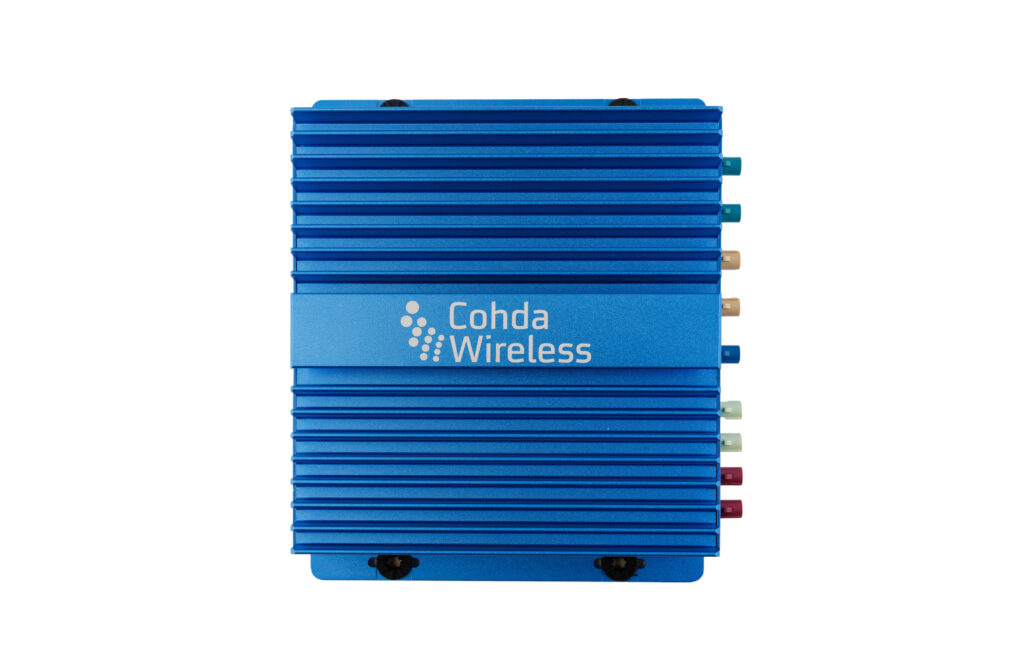
\includegraphics[width=0.76\linewidth,height=0.18\textheight,keepaspectratio]{cohda_mk6_obu.jpg}\par
      \vspace{0.05cm}
      {\color{BrandBlue}\fontsize{11.5}{13.5}\selectfont\bfseries Cohda Wireless MK6 OBU}\par
      \vspace{0.10cm}
      {\raggedright\fontsize{7.6}{9.1}\selectfont
      \begin{itemize}
        \item DSRC and C-V2X, plus 5G cellular, Wi-Fi and Bluetooth
        \item OmniAir, FCC, CE, E1 R10/R118 and other listed certifications
      \end{itemize}}
    \end{column}
    \begin{column}{0.47\textwidth}
      \centering
      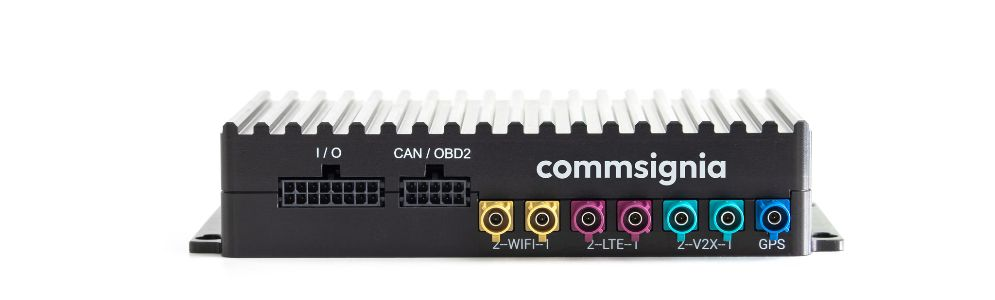
\includegraphics[width=0.88\linewidth,height=0.18\textheight,keepaspectratio]{commsignia_obu.jpg}\par
      \vspace{0.05cm}
      {\color{BrandBlue}\fontsize{11.5}{13.5}\selectfont\bfseries Commsignia OB4}\par
      \vspace{0.10cm}
      {\raggedright\fontsize{7.6}{9.1}\selectfont
      \begin{itemize}
        \item Dual-mode DSRC/C-V2X, GNSS, WLAN/LTE, CAN and GPIO
        \item Onboard sensor inputs, integrated HSM, secure boot and automotive-grade design
      \end{itemize}}
    \end{column}
  \end{columns}
  \vspace{0.03cm}
  {\color{BrandMagenta}\rule{0.08cm}{0.55cm}}\hspace{0.12cm}%
  \begin{minipage}[b]{0.90\linewidth}
    {\fontsize{7.9}{9.5}\selectfont\bfseries Product lesson:} {\fontsize{7.9}{9.5}\selectfont multi-radio V2X, vehicle I/O, positioning, hardware-backed security, protected power, enclosure and lifecycle tools surround the research trust layer.}
  \end{minipage}
  \sourcefoot{Official Cohda Wireless MK6 and Commsignia OBU product pages}
  \note{[Sources]\par
    Cohda Wireless MK6 product page and image: https://cohdawireless.com/solutions/mk6/ and https://cohdawireless.com/wp-content/uploads/2025/02/MK6-OBU-Hero-front-1-scaled.jpg\par
    Commsignia OBU product page and product image: https://commsignia.com/products/obu\par
    Product-envelope statement is an inference from the capabilities listed by both vendors; it is not a direct performance comparison.}
\end{frame}

% -----------------------------------------------------------------------------
\begin{frame}{The next board revision closes four product gaps}
  \begin{columns}[T,onlytextwidth]
    \begin{column}{0.37\textwidth}
      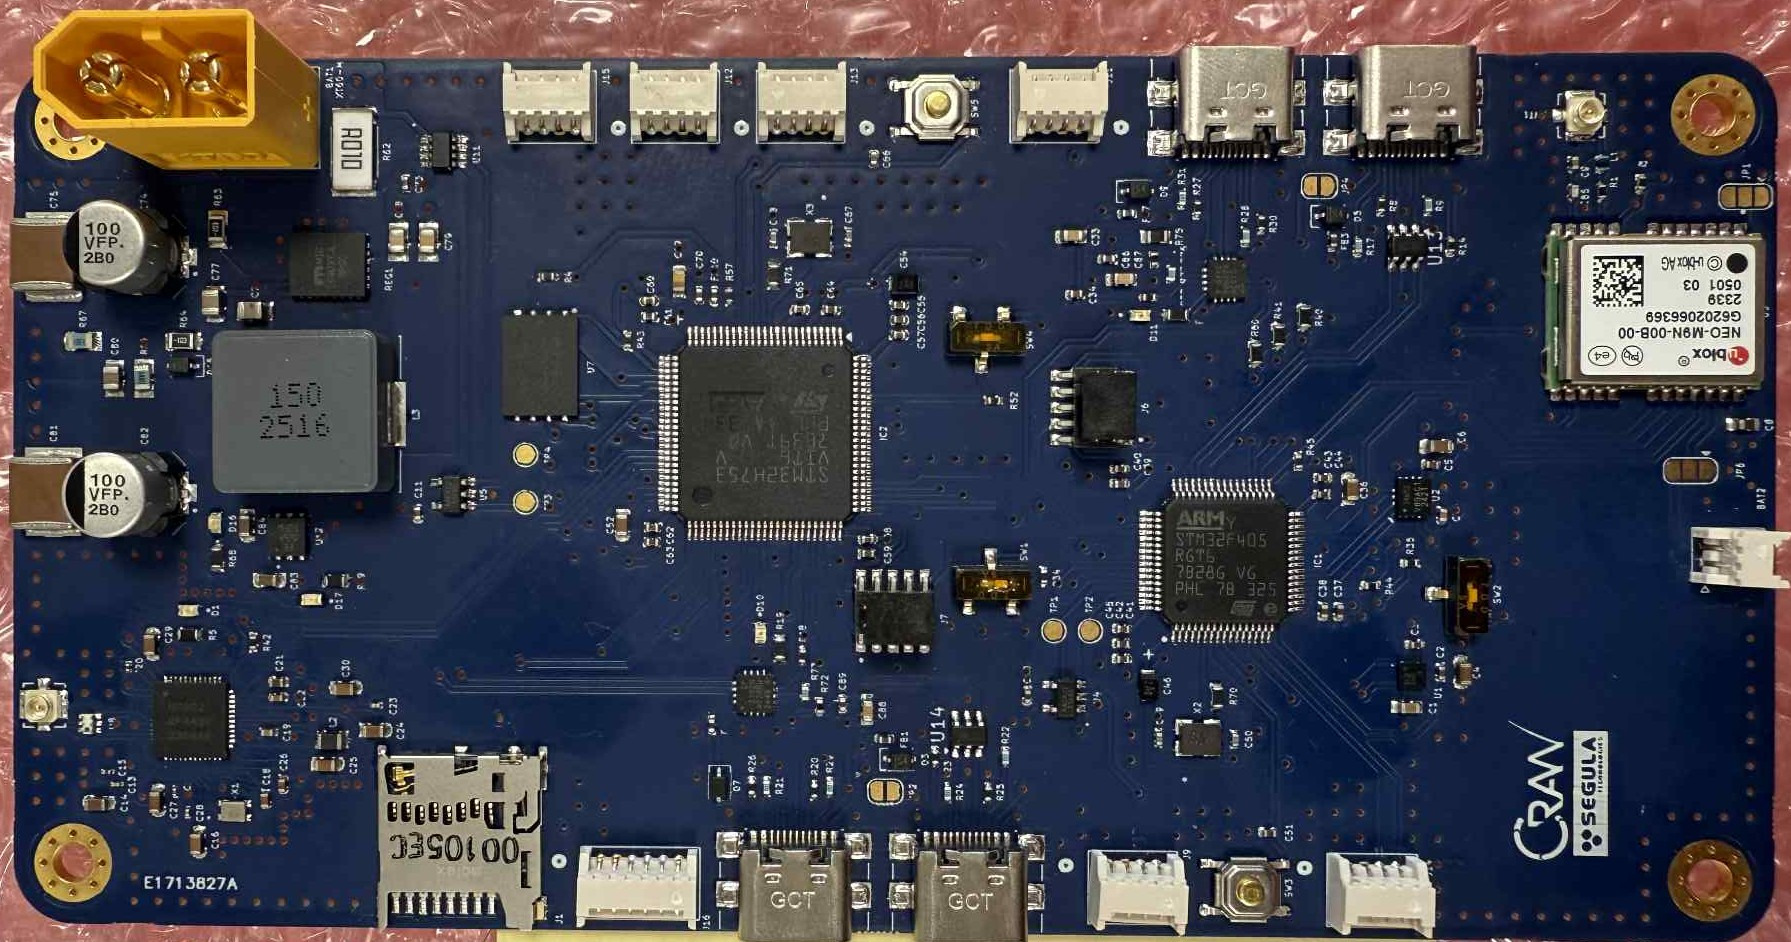
\includegraphics[width=\linewidth,height=0.27\textheight,keepaspectratio]{pcb_photo.jpg}\par
      \vspace{0.08cm}
      {\color{BrandBlue}\fontsize{11.3}{13.4}\selectfont\bfseries Research PCB}\par
      {\color{Muted}\fontsize{7.5}{9}\selectfont Keep the trust, rollback and logging software; redesign the surrounding hardware for the vehicle.}\par
      \vspace{0.11cm}
      {\color{BrandMagenta}\fontsize{9}{10.8}\selectfont\bfseries Deployment principle}\par
      {\fontsize{7.6}{9.2}\selectfont Begin monitor-only behind a gateway before any fallback request is authorized.}
    \end{column}
    \begin{column}{0.57\textwidth}
      \eyebrow{Production-oriented revision}
      \stepnumber{01}\hspace{0.12cm}{\fontsize{9.7}{11.6}\selectfont\bfseries Protected power and enclosure}\par
      {\color{Muted}\fontsize{7.1}{8.5}\selectfont 12/24 V protection, thermal design, automotive components, EMC and environmental validation.}\par
      \vspace{0.08cm}
      \stepnumber{02}\hspace{0.12cm}{\fontsize{9.7}{11.6}\selectfont\bfseries Vehicle and V2X interfaces}\par
      {\color{Muted}\fontsize{7.1}{8.5}\selectfont CAN/CAN-FD or gateway diagnostics and an external or integrated C-V2X/NR-V2X modem.}\par
      \vspace{0.08cm}
      \stepnumber{03}\hspace{0.12cm}{\fontsize{9.7}{11.6}\selectfont\bfseries Sensors and timing}\par
      {\color{Muted}\fontsize{7.1}{8.5}\selectfont Automotive IMU, GNSS/1PPS and selected bus signals; optional vehicle-supplied wheel speed, yaw or pose.}\par
      \vspace{0.08cm}
      \stepnumber{04}\hspace{0.12cm}{\fontsize{9.7}{11.6}\selectfont\bfseries Security and lifecycle}\par
      {\color{Muted}\fontsize{7.1}{8.5}\selectfont Secure boot, signed updates, HSM/secure element, protected logs, keys and update tooling.}
    \end{column}
  \end{columns}
  \sourcefoot{Thesis Chapter 6 roadmap; commercial OBU product capabilities}
  \note{[Sources]\par
    \texttt{\detokenize{ch6/ch6_main.tex}}, integration roadmap and future hardware requirements.\par
    Cohda Wireless MK6 product page: https://cohdawireless.com/solutions/mk6/\par
    Commsignia OBU product page: https://commsignia.com/products/obu\par
    Optional sensor examples are proposed integration inputs, not claims about the present PCB.}
\end{frame}

% -----------------------------------------------------------------------------
\begin{frame}{Research contribution and product readiness are different questions}
  \eyebrow{Positioning}
  \begin{columns}[T,onlytextwidth]
    \begin{column}{0.47\textwidth}
      {\color{Good}\rule{\linewidth}{0.09cm}}\par
      \vspace{0.12cm}
      {\color{Good}\fontsize{12.5}{14.5}\selectfont\bfseries What the research demonstrates}\par
      \vspace{0.10cm}
      {\fontsize{8.6}{10.3}\selectfont
      \begin{itemize}
        \item Trust-adaptive V2V fusion instead of fixed source reliability
        \item Suppression plus rollback/anchoring for future and stored contamination
        \item Nonlinear 2D platoon tests with local and global channel attacks
        \item Trusted estimates exposed to a control-availability decision
      \end{itemize}}
    \end{column}
    \begin{column}{0.47\textwidth}
      {\color{Warn}\rule{\linewidth}{0.09cm}}\par
      \vspace{0.12cm}
      {\color{Warn}\fontsize{12.5}{14.5}\selectfont\bfseries What a product must still prove}\par
      \vspace{0.10cm}
      {\fontsize{8.6}{10.3}\selectfont
      \begin{itemize}
        \item Automotive interfaces, timing and runtime reliability
        \item ISO/SAE 21434 cybersecurity evidence and secure lifecycle
        \item ISO 26262 safety concept when control can be influenced
        \item EMC, environmental, manufacturing and vehicle qualification
      \end{itemize}}
    \end{column}
  \end{columns}
  \vspace{0.10cm}
  {\color{BrandBlue}\rule{0.08cm}{0.52cm}}\hspace{0.12cm}%
  \begin{minipage}[b]{0.90\linewidth}
    {\fontsize{8.2}{9.8}\selectfont\bfseries Current position:} research-validated and hardware-demonstrated, but not yet an automotive-qualified OBU or RSU.
  \end{minipage}
  \sourcefoot{Final manuscript related work; Thesis Chapter 6; ISO/SAE 21434; UNECE R155; ISO 26262}
  \note{[Sources]\par
    \texttt{\detokenize{ch5/TRust_final/manuscript_v7_submit.tex}}, Related Work and Motivation; validation layers and limitations.\par
    \texttt{\detokenize{ch6/ch6_main.tex}}, Architectural alignment with state of the art.\par
    ISO/SAE 21434:2021: https://www.iso.org/standard/70918.html\par
    UNECE UN Regulation No. 155: https://unece.org/transport/documents/2021/03/standards/un-regulation-no-155-cyber-security-and-cyber-security\par
    ISO 26262 series: https://www.iso.org/publication/PUB200262.html}
\end{frame}

% -----------------------------------------------------------------------------
\begin{frame}{How SEGULA can reuse the work}
  \eyebrow{Engineering value across customer programs}
  \vspace{0.06cm}
  \begin{columns}[T,onlytextwidth]
    \begin{column}{0.30\textwidth}
      \stepnumber{01}\par\vspace{0.09cm}
      {\fontsize{12}{14}\selectfont\bfseries Reusable assets}\par
      \vspace{0.13cm}
      {\color{Muted}\fontsize{8.4}{10.1}\selectfont Trust and rollback software, embedded reference design, repeatable attacks, digital-twin scenarios and synchronized logs.}
    \end{column}
    \begin{column}{0.30\textwidth}
      \stepnumber{02}\par\vspace{0.09cm}
      {\fontsize{12}{14}\selectfont\bfseries Client work packages}\par
      \vspace{0.13cm}
      {\color{Muted}\fontsize{8.4}{10.1}\selectfont V2X-resilience studies, HW/SW integration, cyber-robustness campaigns and safety, EMC or vehicle-validation support.}
    \end{column}
    \begin{column}{0.30\textwidth}
      \stepnumber{03}\par\vspace{0.09cm}
      {\fontsize{12}{14}\selectfont\bfseries Value to test}\par
      \vspace{0.13cm}
      {\color{Muted}\fontsize{8.4}{10.1}\selectfont Less repeated setup, a differentiated OEM/Tier-1 offer and follow-on engineering through integration and industrialization.}
    \end{column}
  \end{columns}
  \vspace{0.26cm}
  {\color{BrandMagenta}\rule{0.08cm}{0.78cm}}\hspace{0.12cm}%
  \begin{minipage}[b]{0.90\linewidth}
    {\fontsize{9}{10.8}\selectfont\bfseries Commercial gate:} confirm customer demand, integration effort, reuse rate and engineering time saved before making an ROI claim.
  \end{minipage}
  \sourcefoot{SEGULA automotive, ADAS, cybersecurity and EMC service positioning; thesis validation assets}
  \note{[Sources]\par
    SEGULA Automotive and industrial vehicles: https://www.segulatechnologies.com/en/industries/automotive-and-industrial-vehicles/\par
    SEGULA Driver assistance systems: https://www.segulatechnologies.com/en/driver-assistance-systems/\par
    SEGULA automotive cybersecurity partnership: https://www.segulatechnologies.com/en/news/segula-technologies-c2a-security-cybersecurite-automobile/\par
    SEGULA Electromagnetic Compatibility: https://www.segulatechnologies.com/en/electromagnetic-compatibility-emc/\par
    \texttt{\detokenize{ch6/ch6_main.tex}}, board motivation, experimental workflow and traceability.\par
    The value proposition is an inference from the documented project assets and SEGULA's published capabilities.}
\end{frame}

% -----------------------------------------------------------------------------
\begin{frame}{Decision requested: launch a monitor-only pilot}
  \begin{columns}[T,onlytextwidth]
    \begin{column}{0.44\textwidth}
      \eyebrow{Recommended next gate}
      {\color{BrandBlue}\fontsize{20}{22.5}\selectfont\bfseries Observe first.\par Measure.\par Then decide.}\par
      \vspace{0.18cm}
      {\fontsize{8.8}{10.6}\selectfont The board calculates trust and recovery decisions and records them, but it does not command the actuators.}\par
      \vspace{0.20cm}
      {\color{BrandMagenta}\rule{\linewidth}{0.09cm}}\par
      \vspace{0.11cm}
      {\color{BrandMagenta}\fontsize{9.2}{11}\selectfont\bfseries Go/no-go evidence}\par
      {\color{Muted}\fontsize{7.7}{9.2}\selectfont False positives, detection delay, packet loss, recovery, compute load and integration effort.}
    \end{column}
    \begin{column}{0.50\textwidth}
      \eyebrow{Conditions to start}
      \stepnumber{01}\hspace{0.14cm}{\fontsize{11}{13}\selectfont\bfseries Vehicle access}\par
      {\color{Muted}\fontsize{8.2}{9.8}\selectfont A target program provides bus access and a measurable cooperative-driving use case.}\par
      \vspace{0.15cm}
      \stepnumber{02}\hspace{0.14cm}{\fontsize{11}{13}\selectfont\bfseries Production-like interfaces}\par
      {\color{Muted}\fontsize{8.2}{9.8}\selectfont Connect the target CAN/CAN-FD gateway and a representative V2X modem.}\par
      \vspace{0.15cm}
      \stepnumber{03}\hspace{0.14cm}{\fontsize{11}{13}\selectfont\bfseries Joint ownership}\par
      {\color{Muted}\fontsize{8.2}{9.8}\selectfont Hardware, software, cybersecurity and safety owners agree on the evidence and stop criteria.}\par
      \vspace{0.18cm}
      {\color{Good}\fontsize{8.2}{9.8}\selectfont\bfseries The pilot decides whether further industrialization is justified.}
    \end{column}
  \end{columns}
  \sourcefoot{Thesis Chapter 6 staged roadmap and SEGULA vehicle-integration capabilities}
  \note{[Sources]\par
    \texttt{\detokenize{ch6/ch6_main.tex}}, Integration roadmap with thesis algorithms and future optimization/stress-test axes.\par
    SEGULA complete-vehicle development: https://www.segulatechnologies.com/en/development-of-complete-vehicles/\par
    SEGULA ADAS development, functional safety, integration and validation: https://www.segulatechnologies.com/en/driver-assistance-systems/\par
    Recommendation is an inference from the documented monitoring-first roadmap, current maturity and SEGULA's published engineering capabilities.}
\end{frame}

\end{document}
